% Created 2020-10-14 Wed 15:40
% Intended LaTeX compiler: pdflatex
\documentclass[11pt]{article}
\usepackage[utf8]{inputenc}
\usepackage[T1]{fontenc}
\usepackage{graphicx}
\usepackage{grffile}
\usepackage{longtable}
\usepackage{wrapfig}
\usepackage{rotating}
\usepackage[normalem]{ulem}
\usepackage{amsmath}
\usepackage{textcomp}
\usepackage{amssymb}
\usepackage{capt-of}
\usepackage{hyperref}
\usepackage{listings}
\usepackage[ruled,vlined]{algorithm2e}
\author{Antonio Caliò}
\date{\today}
\title{Data Model}
\hypersetup{
 pdfauthor={Antonio Caliò},
 pdftitle={Data Model},
 pdfkeywords={},
 pdfsubject={},
 pdfcreator={Emacs 27.1 (Org mode 9.3)}, 
 pdflang={English}}
\begin{document}

\maketitle

\section{Comment}
\label{sec:org25e3f20}
\begin{enumerate}
\item Definition
\label{sec:org10d22c9}
\begin{center}
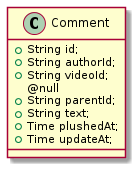
\includegraphics[width=.9\linewidth]{comment.png}
\end{center}

\item Api Call
\label{sec:orgab9711d}

In the following snippet there is an example of API call result.

More specifically given a \texttt{parentId}, this is the result containing all the 
comments that replies to the comment pointed by \texttt{commentId}.
\end{enumerate}
\section{My Api}
\label{sec:org0b7a04e}
In this section we describe how to use our custom API, built around the Youtube-Api, in order to
extract all the significant information related to our application.

Data are required in order to build the following knowledge system.

\begin{itemize}
\item Comments/Replies Graph
\item LikeGraph
\item Subscription Graph -- it might be subject to some YouTube restrictions
\end{itemize}


\begin{enumerate}
\item Pipeline for the Comments/Replies Graph
\label{sec:org8a78a8c}

Below is the high-level algorithm for extractng the Comments/Replies 
required to build the final graph.

\begin{latex}
\begin{algorithm}[H]
\SetAlgoLined
\KwIn{A query Q, Number of videos to be processed N}
 
 Execute Query Q get first N related videos\;	
 \ForEach{video} {
     store(video)\;		 
     comments \gets API.commentthread(video.id)\;
     \ForEach{comment)}{
        store(comment)\;
	\If(comment.replies.length>0){
	  replies \gets API.comment(parentid=comment.id)\;
	  \ForEach{reply in replies}{
	     store(reply)
	  }
	}	
     }			 
 }
 
\caption{Given a Query }
\end{algorithm}
\end{latex}
\end{enumerate}
\end{document}